% A loop gamma based at x_0 in a space X.
% Source: book/tex/topology/fundamental-group.tex (§ Fundamental groups).
\documentclass[border=2mm]{standalone}
\usepackage{tikz}
\usetikzlibrary{arrows.meta,decorations.markings}
\begin{document}
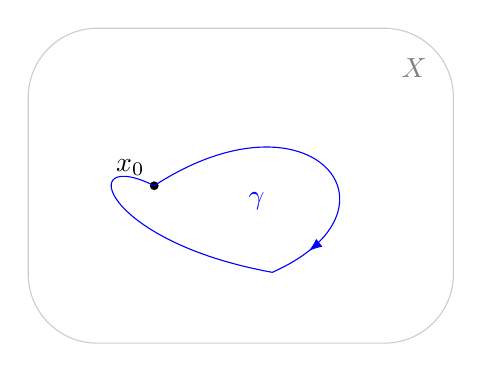
\begin{tikzpicture}[scale=1]
  \draw[rounded corners=25pt, gray!40] (-2.6,-2) rectangle (2.8,2);
  \node[gray] at (2.3,1.5) {$X$};
  \fill (-1,0) circle (1.6pt) node[above left] {$x_0$};
  \draw[blue,decoration={markings,mark=at position 0.5 with {\arrow{Latex}}},
    postaction={decorate}]
    (-1,0) .. controls (1,1.3) and (2.3,-0.3) .. (0.5,-1.1)
           .. controls (-1.7,-0.7) and (-2,0.5) .. (-1,0);
  \node[blue] at (0.3,-0.2) {$\gamma$};
\end{tikzpicture}
\end{document}
